\documentclass{article}
\usepackage{makecell}
\usepackage{graphicx}
\usepackage{geometry}
\usepackage{multirow}
\usepackage{multicol}
\usepackage{fancyhdr}
\usepackage{longtable}
\usepackage{color}
\usepackage{float}
\usepackage{listings}
\usepackage{xcolor}
\usepackage{hyperref}
\usepackage{paralist}
\usepackage{pifont}
\usepackage{amsmath}
\usepackage{booktabs}
\usepackage{amssymb}
\usepackage{wrapfig}
\usepackage{caption}
\usepackage{pgf}
\usepackage{tikz}
\usetikzlibrary{arrows,automata}
\usepackage[ruled,linesnumbered]{algorithm2e}

\SetKw{Continue}{continue}
\SetKw{True}{True}
\SetKw{False}{False}

\newcommand{\tabitem}{~~\llap{\textbullet}~~}
\renewcommand{\labelitemii}{\textbullet}
\renewcommand{\labelitemiii}{\textbullet}
\captionsetup{labelfont=bf}

\let\itemize\compactitem
\let\enditemize\endcompactitem
\let\enumerate\compactenum
\let\endenumerate\endcompactenum
\let\description\compactdesc
\let\enddescription\endcompactdesc

\setlength{\lineskip}{2.5pt}
\setlength{\lineskiplimit}{2.5pt}

\geometry{a4paper,left=25mm,right=20mm,top=25mm,bottom=25mm}

\pagestyle{fancy}
\fancyhead[L]{}
\fancyhead[R]{\thepage}
\fancyfoot[L]{}
\fancyfoot[C]{}
\fancyfoot[R]{}
\renewcommand{\headrulewidth}{0pt}

\title{JLex: A Simple Lex Implementation}
\author{09021227~Jin Qiao}
\date{\today}

\lstset{
    numbers=left,
    keywordstyle= \color{ blue!70},
    commentstyle= \color{red!50!green!50!blue!50},
    rulesepcolor= \color{ red!20!green!20!blue!20} ,
    % escapeinside=``,
    numberstyle=\tt,
    numbersep=0em,
    xleftmargin=2em,
    breaklines,
    aboveskip=1em,
    framexleftmargin=2em,
    frame=shadowbox,
    basicstyle=\tt,
    language=C++
}

\begin{document}

\begin{titlepage}
    \hfill\includegraphics[width=2cm]{img/seu-logo.pdf}

    \vspace*{8cm}

    {\huge\textbf{JLex}}

    \vspace*{0.5em}

    {\Large{A Simple Lex Implementation}}

    \vspace*{1em}

    {\large {09021227~Jin Qiao}}
\end{titlepage}

\tableofcontents
\newpage

\section{Motivation \& Aim}

\textit{lex} is one of the most used lexical analyzer today and it is usually used with \textit{yacc} to generate programs for those who want to write compilers or intepreters. For lex, you only need to write regular expressions and lex will generate corresponding lexical analyzer program. One of the most used implementation of lex is flex and one of the most used implementation of yacc is bison. Both of them are open-sourced and based on BSD license.

According to the description of the experiment, we are going to implement a simple lexical analyzer, which is like flex. It reads regular expressions defined by user and generate corresponding lexical analyzer program. We also need to define our \texttt{.l} file, where stores the regular expressions.

Therefore, introducing \textbf{JLex}, which is short for \textbf{J}inbridge-\textbf{Lex}ical-Analyzer. (Actually, JinBridge is my nickname). It mainly has following features:

\begin{itemize}
    \item Nearly the same interface with \textit{lex}. The \texttt{.l} file used by \textbf{JLex} is very similar to that used by \textit{lex}, with only little change.
    \item Support escape characters, \textit{e.g.} \texttt{\textbackslash t}, \texttt{\textbackslash n}.
    \item Created with C\texttt{++}11.
\end{itemize}

Anyway, I shall not spend too much time here, let's just get into the main topic.

\section{Ideas \& Methods}

For the main idea and method, I'll just use algorithm discussed on class to keep this project as simple as possible. The program includes two part: the \textit{JLex} itself and the \texttt{source.cpp} file.

Actually, I didn't read the source code of \textit{lex} and I used a very dummy implementation, which is to replace text content of a prepared C\texttt{++} program. The prepared C\texttt{++} program is \texttt{source.cpp} file and \textit{JLex} will replace the content of \texttt{source.cpp} to generate corresponding lexical analyzer. Here I draw a simple diagram in Fig.~\ref{jlex-process} to explain how it works.

\begin{figure}[htpb]
    \centering
    \includegraphics[width=0.7\textwidth]{img/jlex-process.pdf}
    \caption{\textbf{The flow chart of JLex.} Almost the same with lex. You just give the \texttt{.l} file to \textit{JLex} and it will generate corresponding \texttt{lex.yy.cpp} file. Compile this source file and you will get the lexical analyzer program. It reads the source code and outputs the analysis result.}
    \label{jlex-process}
\end{figure}

The \texttt{source.cpp} file is prepared and all \textit{JLex} do is to replace the content in it. So I will not spend too much time on replacing algorithm in \textit{JLex} and instead, I'll introduce the content in \texttt{source.cpp}.

\section{Content Description}

A simple \textit{lex} implementation written in C\texttt{++}. Source code available on \href{https://github.com/JinBridger/SEU-Compiler-Labwork}{\textcolor{blue}{\texttt{\underline{here}}}}.

\section{Assumptions}

\subsection{Regular Expression Format}

To keep the project simple, I'll not implement all operators in \textit{lex} regular expression format. Instead, the regular expression in \textit{JLex} including following operators: \texttt{(, ), *, |, @}, which is listed in Table~\ref{operator}.

The first three operators are the same with corresponding symbol in textbook. Note that the fourth symbol, which is \texttt{@}. It connects two factors and usually we just ignore it. For example, we always write $a\times b$ as $ab$ and we just skip times symbol. When we write regular expression, we also ignore the connect operator and write \texttt{a@b} as \texttt{ab}.

\begin{table}[htbp]
    \centering
    \begin{tabular}{cccc}
        \toprule
        \textbf{Operator} & \textbf{Name} & \textbf{Priority} & \textbf{Example}                   \\
        \midrule
        \texttt{()}       & Parentheses   & 0                 &                                    \\
        \texttt{*}        & Kleene star   & 1                 & \texttt{ab* = \{a, ab, abb, ...\}} \\
        \texttt{|}        & Or            & 2                 & \texttt{a|b = \{a, b\}}            \\
        \texttt{@}        & Connect       & 3                 & \texttt{a@b = \{ab\}}              \\
        \bottomrule
    \end{tabular}%
    \caption{\textbf{Operators used in \textit{JLex}.}}
    \label{operator}%
\end{table}%

Based on this 4 operators, we could express almost all the regular expressions. However, it's still not convenient. For example, if we want to express from A to Z, we must write \texttt{A|B|C|...|Z}. To make it easier to write regular expression, I defined following marcos: \texttt{A-Z}, \texttt{a-z}, \texttt{0-9}. The usage is the same with in \textit{lex}. You could just write \texttt{(a-z)} to match all alphabets.


To match special characters such as \texttt{\textbackslash n} and \texttt{\textbackslash t}, it also support escape characters. Also, when you use \texttt{\textbackslash (} in the regular expression, the \texttt{(} will be treated as a character. This is also suitable for \texttt{*}, \texttt{|} and \texttt{@}.

\subsection{\texttt{.l} File Format}

The \texttt{.l} file for \textit{JLex} is relatively similar to that for \textit{lex}. The \texttt{yylex()}, \texttt{yytext} and \texttt{yyin} is still available in \textit{JLex}. The difference is:
\begin{itemize}
    \item \textit{JLex} uses \texttt{→} to separate regular expression and the action.
    \item \textit{JLex} does not have definition section.
\end{itemize}
However, \textit{JLex} still supports inserting code at the beginning of generated C\texttt{++} code.

Here I give a simple example of \texttt{.l} file for \textit{JLex}. It simply matches the integers in the text.

\begin{lstlisting}
    %{
        // any code here will be inserted to the beginning of lex.yy.cpp
        #include <iostream>
    %}
    
    %%

    (0-9)* →  { std::cout << "integer: " + yytext << std::endl; }
    
    %%
    
    // any code here will be inserted to the end of lex.yy.cpp
    int main(int argc, char** argv) {
        yyin = argv[1];
        yylex();
        return 0;
    }
\end{lstlisting}

An example of matching C language tokens will be given in \textit{Use Cases on Running}.

\section{Related FA Descriptions}

Here I define two kinds of FA: static FA and runnable FA. Static FA is used to calculate and runnable FA is used to match tokens. We first calculate a static FA and then load it in a runnable FA to run.

\subsection{Static FA}
Here I'll show how I define static finite-state automaton (FA) in code.

Actually, the FA stores a graph, where nodes are states and edges are transition. I use adjacency list to store the graph because the FA is a sparse graph. I'll introduce adjacency list in \textit{Description of Important Data Structures}. For each edge in graph, I store three attributes: \texttt{\_to}, \texttt{\_next}, \texttt{\_ch}. The first two attributes are used for adjacency list and the third attribute \texttt{\_ch} is used to store the character for transition. Note that I use \texttt{@} to express $\varepsilon$.

Besides the graph, some other attributes also needed to be stored in FA:
\begin{itemize}
    \item total states of FA.
    \item the set of all symbols of FA. This is used for simplify NFA to DFA and minimize DFA.
    \item the acceptable states of FA and the corresponding token.
\end{itemize}

Also, I add a simple debug function to print the content in FA. It will print every edge of the FA and outputs the acceptable states in FA.

Below is the \texttt{fa} struct. Here I misused the \textit{status} and \textit{state}. But actually, they are the same meanings in my code.

\begin{lstlisting}
    // actually, it is a graph
    // use '@' for epsilon
    struct fa {
        fa(int total_status) : _total_status(total_status), _head(std::vector<int>    (total_status, -1)) {
            for (int i = 0; i < total_status; ++i) {
                _accept_status[i] = -1;
            }
        }
    
        int _total_status = 0;
        // start status is default 0
        // for nfa, accept status is total status - 1
        // for dfa, accept status is _accept_status
    
        struct edge {
            int  _to, _next;
            char _ch;
        };
        std::vector<int>  _head;
        std::vector<edge> _edge;
    
        std::set<char> _symbols;
        // std::set<int>      _accept_status;
        // key: status, value: token enum in int
        std::map<int, int> _accept_status;
    
        void add_edge(int from, int to, char c) {
            _edge.push_back(edge());
            _edge[_edge.size() - 1]._to   = to;
            _edge[_edge.size() - 1]._ch   = c;
            _edge[_edge.size() - 1]._next = _head[from];
            _head[from]                   = _edge.size() - 1;
        }
    
        void print() {
            for (int i = 0; i < _total_status; ++i) {
                if (_head[i] == -1)
                    continue;
                std::cout << "Status " + std::to_string(i) << std::endl;
                for (int idx = _head[i]; idx != -1; idx = _edge[idx]._next)
                    std::cout << "    --" << _edge[idx]._ch << "--> " << std::to_string(_edge    [idx]._to) << std::endl;
            }
            std::cout << "Accept states:" << std::endl;
            for (auto i : _accept_status)
                std::cout << "    " << i.first << ": " << i.second << std::endl;
        }
    };
\end{lstlisting}

\subsection{Runnable FA}

After we calculate a static FA, we need to load it into a runnable FA. Compared to static FA, the runnable FA stores current state, and it supports input characters. Also, it supports you to reset it.

\begin{lstlisting}
    struct runnable_fa {
        runnable_fa(fa f) : _fa(f), _current_state(0) {}
        fa  _fa;
        int _current_state;
        // return value:
        // false: failed, true: find
        bool input(char ch) {
            for (int i = _fa._head[_current_state]; i != -1; i = _fa._edge[i]._next) {
                if (_fa._edge[i]._ch == ch) {
                    _current_state = _fa._edge[i]._to;
                    return true;
                }
            }
            return false;
        }
    
        void reset() {
            _current_state = 0;
        }
    };
\end{lstlisting}

\section{Description of Important Data Structures}

\subsection{Adjacency List}

Adjacency list is used to store a graph, especially a sparse graph. It includes following parts:
\begin{itemize}
    \item \texttt{head} array, which stores the index of first edge from the node. For example, \texttt{head[i]} is the index of first edge from node \texttt{i}.
    \item \texttt{edge} array, which stores the information of edges.
    \item the number of total edges.
\end{itemize}

For each edge, it has three attributes:
\begin{itemize}
    \item \texttt{next}, stores the index of next edge which starts from the same node.
    \item \texttt{to}, stores the destination of the edge.
\end{itemize}

I'll not explain the algorithms used to add edge and iterate edges because they are not important, and you could easily get more detailed explanation about them on Google.

\subsection{Containers of STL}

To simplify the project, I used some containers in STL:
\begin{itemize}
    \item \texttt{std::vector}, it's time to throw traditional array away.
    \item \texttt{std::stack}, a STL implementation of stack.
    \item \texttt{std::set}, stores a set where there are no two same elements.
    \item \texttt{std::string}, stores the string.
    \item \texttt{std::function}, stores the function when match a specific regular expression. I used it together with lambda expression of C\texttt{++}11.
\end{itemize}

Also, I'll not explain them here because a more detailed explanation could be found in CppReference.

\section{Description of Core Algorithm}

The core algorithms are the same with those on textbook. I'll introduce them according to the sequence of I used them.

\subsection{Convert Regular Expression to NFA}

For this part, the main task is to convert the given regular expression to NFA. Note that before we actually convert it, we need to expand the macros like \texttt{a-z}, and read the escaped characters like \texttt{\textbackslash (}. Also, we need to complete all connect operators we ignored before.

After we applied these three steps on given regular expression, we then convert the regular expression from infix expression to postfix expression so that we could process it with a stack.

Here's the algorithm to convert infix expression to postfix expression, which is Algorithm~\ref{convert-infix}.

\begin{algorithm}
    \caption{Convert infix regular expression to postfix regular expression}
    \label{convert-infix}
    \KwIn{Infix regular expression $R$}
    \KwOut{Postfix regular expression $R'$}
    Let $O$ be the operator stack.\\
    Let $I$ be the intermediate stack.\\
    \For{$i \leftarrow 0$ \KwTo R's length}{
        \If{$R[i]$ is not operator}{
            Push $R[i]$ into $I$.\\
            \Continue
        }

        \If{$R[i]$ is operator}{
            \If{$O$ is empty or the top of $O$ is (}{
                Push $R[i]$ into $O$.\\
                \Continue
            }
            \While{priority of the top of $O$ is higher than $R[i]$}{
                Push the top of $O$ into $I$.\\
                Pop the top of $O$.\\
            }
            \If{priority of the top of $O$ is lower than $R[i]$}{
                Push $R[i]$ into $O$.\\
                \Continue
            }
        }

        \If{$R[i]$ is (}{
            Push $R[i]$ into $O$.\\
            \Continue
        }
        \If{$R[i]$ is )}{
            \While{the top of O is not (}{
                Push the top of $O$ into $I$.\\
                Pop the top of $O$.
            }
            Pop the top of $O$.\\
            \Continue
        }
    }
    Push elements in $O$ into $I$ one by one.\\
    Let $R'$ be the reverse of elements in $I$.\\
    \Return{$R'$}
\end{algorithm}

After we convert the infix regular expression to postfix regular expression, we could calculate the NFA of it just like the way we calculate value of postfix expression. We will use a stack to calculate the NFA of it.

Note that for each of character, we will generate a NFA for it. For example, for character \texttt{s} we will generate following NFA for it:、

\begin{center}
    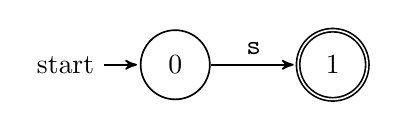
\begin{tikzpicture}[->,>=stealth',shorten >=1pt,auto,node distance=2cm,
            semithick]
        \tikzstyle{every state}=[draw=black,text=black]

        \node[initial,state] (A) {0};
        \node[state, accepting] (B) [right of=A] {1};

        \path (A) edge node {\texttt{s}} (B);
    \end{tikzpicture}
\end{center}

When we combine two NFAs with operator \texttt{|}, for example a NFA for \texttt{a|b}, we will generate following NFA:

\begin{center}
    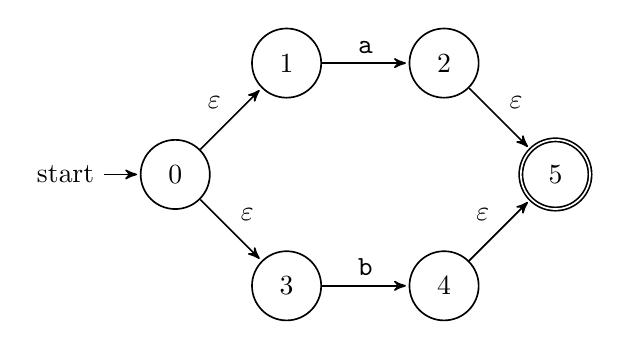
\begin{tikzpicture}[->,>=stealth',shorten >=1pt,auto,node distance=2cm,
            semithick]
        \tikzstyle{every state}=[draw=black,text=black]

        \node[initial,state] (E) {0};
        \node[state] (A) [above right of=E] {1};
        \node[state] (B) [right of=A] {2};
        \node[state] (C) [below right of=E] {3};
        \node[state] (D) [right of=C] {4};
        \node[state, accepting] (F) [below right of=B] {5};

        \path (E) edge node {$\varepsilon$} (A);
        \path (E) edge node {$\varepsilon$} (C);
        \path (B) edge node {$\varepsilon$} (F);
        \path (D) edge node {$\varepsilon$} (F);
        \path (A) edge node {\texttt{a}} (B);
        \path (C) edge node {\texttt{b}} (D);
    \end{tikzpicture}
\end{center}

When we combine two NFAs with operator \texttt{@}, for example, a NFA for \texttt{a@b}, we will generate following NFA:

\begin{center}
    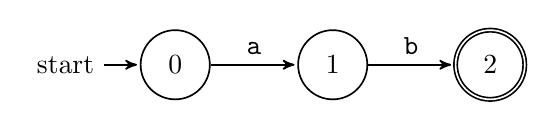
\begin{tikzpicture}[->,>=stealth',shorten >=1pt,auto,node distance=2cm,
            semithick]
        \tikzstyle{every state}=[draw=black,text=black]

        \node[initial,state] (E) {0};
        \node[state] (A) [right of=E] {1};
        \node[state, accepting] (B) [right of=A] {2};

        \path (E) edge node {\texttt{a}} (A);
        \path (A) edge node {\texttt{b}} (B);
    \end{tikzpicture}
\end{center}

When we use operator \texttt{*}, for example, a NFA for \texttt{a*}, we will generate following NFA:

\begin{center}
    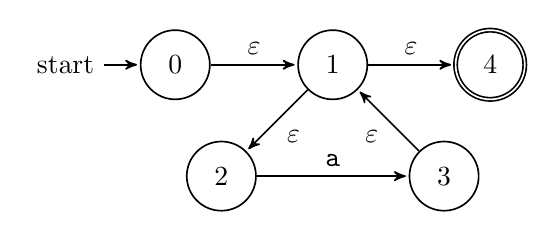
\begin{tikzpicture}[->,>=stealth',shorten >=1pt,auto,node distance=2cm,
            semithick]
        \tikzstyle{every state}=[draw=black,text=black]

        \node[initial, state] (S) {0};
        \node[state] (T) [right of=S] {1};
        \node[state, accepting] (E) [right of=T] {4};

        \node[state] (A) [below left of=T] {2};
        \node[state] (B) [below right of=T] {3};

        \path (S) edge node {$\varepsilon$} (T);
        \path (T) edge node {$\varepsilon$} (E);
        \path (T) edge node {$\varepsilon$} (A);
        \path (B) edge node {$\varepsilon$} (T);

        \path (A) edge node {\texttt{a}} (B);
    \end{tikzpicture}
\end{center}

After we define actions for these operators, we are able to introduce the algorithm to generate the NFA, which is Algorithm~\ref{convert-postfix-to-NFA}.

\begin{algorithm}
    \caption{Convert postfix regular expression to NFA}
    \label{convert-postfix-to-NFA}
    \KwIn{Postfix regular expression $R$}
    \KwOut{Corresponding NFA $N$}
    Let $S$ be a stack.\\
    \For{$i \leftarrow 0$ \KwTo R's length}{
        \uIf{R[i] is an operator}{
            Get the top two elements in $S$ and remove them in $S$.\\
            Perform corresponding operation on these two elements.\\
            Push the result into $S$.
        }
        \Else{
            Generate corresponding NFA and push it into $S$.
        }
    }
    \Return{$R'$}
\end{algorithm}

Therefore, we could convert each regular expression to corresponding NFA. The next problem is how to combine these NFAs to become a big NFA. The idea is very simple, just add a common start and let it point to the start of those NFAs. For example, if we have NFA for \texttt{a} and \texttt{b}, we could combine them in this way:

\begin{center}
    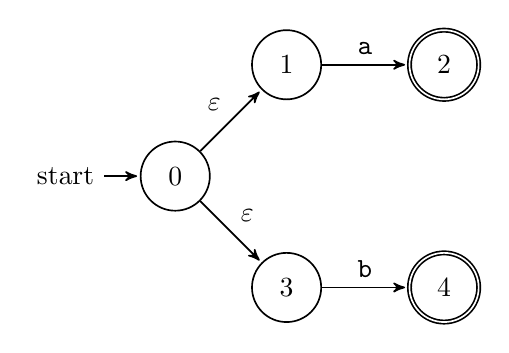
\begin{tikzpicture}[->,>=stealth',shorten >=1pt,auto,node distance=2cm,
            semithick]
        \tikzstyle{every state}=[draw=black,text=black]

        \node[initial,state] (E) {0};
        \node[state] (A) [above right of=E] {1};
        \node[state, accepting] (B) [right of=A] {2};
        \node[state] (C) [below right of=E] {3};
        \node[state, accepting] (D) [right of=C] {4};

        \path (E) edge node {$\varepsilon$} (A);
        \path (E) edge node {$\varepsilon$} (C);
        \path (A) edge node {\texttt{a}} (B);
        \path (C) edge node {\texttt{b}} (D);
    \end{tikzpicture}
\end{center}

The algorithm for this action is shown in Algorithm~\ref{combine-NFAs}.

\begin{algorithm}
    \caption{Combine NFAs to become a big NFA}
    \label{combine-NFAs}
    \KwIn{NFAs $N_1, N_2, ..., N_m$}
    \KwOut{Combined NFA $N$}
    Let $N$ be an empty FA.\\
    Add dummy state 0 to $N$.\\
    \ForEach{$N_i$ in NFAs}{
        Copy $N_i$ to $N$.\\
        Add an edge from 0 to the start of $N_i$.
    }
    \Return{$N$}
\end{algorithm}

\subsection{Convert NFA to DFA}

The next step is to convert the combined NFA to DFA. Here I just use the algorithm in textbook, which is shown in Algorithm~\ref{convert-NFA-to-DFA}.

\begin{algorithm}
    \caption{Convert NFA to DFA}
    \label{convert-NFA-to-DFA}
    \KwIn{NFA $N$}
    \KwOut{Corresponding DFA $D$}
    Initially, $\varepsilon\text{-}closure(s_0)$ is the only state in $D$, and it is unmarked.\\
    \While{there is an unmarked state T in D}{
        Mark $T$.\\
        \ForEach{input symbol a}{
            Let $U$ be $\varepsilon\text{-}closure(move(T, a))$.\\
            \If{U is not in D}{
                Add $U$ as an unmarked state to $D$.
            }
            Add an edge from $T$ to $U$ with char $a$.
        }
    }
    \Return{$D$}
\end{algorithm}

\subsection{Minimize DFA}

In order to make the program run faster, we need to minimize the states in DFA. Here I also used the algorithm in textbook, which is shown in Algorithm~\ref{minimize-dfa}.

\begin{algorithm}
    \caption{Minimize DFA}
    \label{minimize-dfa}
    \KwIn{DFA $D$}
    \KwOut{Corresponding minimized DFA $D'$}
    Construct an initial partition $\Pi$ with two groups $F$ and $S-F$.\\
    Let $\Pi_\text{new}$ be empty.\\
    \While{$\Pi_\text{new}$ not equals to $\Pi$}{
        Let $\Pi_\text{new}$ equals to $\Pi$.\\
        \ForEach{group G in $\Pi$}{
            Partition $G$ into subgroups such that two states $s$ and $t$ are in the same subgroup if and only if for all input symbol $a$, state $s$ and $t$ have transitions on $a$ to states in the same group of $\Pi$.\\
            Replace $G$ in $\Pi_\text{new}$ by the set of all subgroups formed.
        }
    }
    Choose one state in each group of $\Pi_\text{final}$ as the \textit{representative} for that group and Construct the rest of DFA by these representatives.\\
    \Return{$D'$}
\end{algorithm}

\subsection{Run DFA on Given Text}

The final part is to run DFA on given text. Again, I used the algorithm in textbook, which is shown in Algorithm~\ref{run-dfa}.

\begin{algorithm}
    \caption{Run DFA on Given Text}
    \label{run-dfa}
    \KwIn{DFA $D$, Given Text $S$}
    \KwOut{A boolean value to show if the progress has error}
    \ForEach{character c in S}{
        \If{c is not in the alphabets of S}{
            \Return{\False}
        }
        Let $s$ be the current state of $D$.\\
        \uIf{s has an edge to s' with character c}{
            Let the current state of $D$ be $s'$.
        }
        \Else{
            \uIf{s is acceptable}{
                Perform corresponding action.\\
                Reset the current state of $D$ to start.\\
                Retry character $c$.
            }
            \Else{
                \Return{\False}
            }
        }
    }
    \Return{\True}
\end{algorithm}

\texttt{regexpr.hpp}, \texttt{nfa.hpp}, \texttt{dfa.hpp}, \texttt{minimize\_dfa.hpp}, \texttt{runner.hpp}, \texttt{lex.hpp} including all algorithm I mentioned above. All these files combined to be \texttt{source.cpp}. What \textit{JLex} does is to replace the content in \texttt{source.cpp}.

\section{Use Cases on Running}

Here's a simple example to recognize the tokens in C language.

\subsection{Input}

\subsubsection{\texttt{example.l}}
Here's the content in \texttt{example.l} file, and it will simply output what it recognized.

\begin{lstlisting}
    %{
        #include <iostream>
        int test = 0;
    %}
    
    %%
    
     ( )*      →  {}
    \n         →  {}
    ;          →  { std::cout << "MATCH: ;" << std::endl; }
    \\(        →  { std::cout << "MATCH: (" << std::endl; }   
    \\)        →  { std::cout << "MATCH: )" << std::endl; }   
    {          →  { std::cout << "MATCH: {" << std::endl; }   
    }          →  { std::cout << "MATCH: }" << std::endl; }
    [          →  { std::cout << "MATCH: [" << std::endl; }   
    ]          →  { std::cout << "MATCH: ]" << std::endl; }
    
    main       →  { std::cout << "MATCH: main" << std::endl; }
    
    auto       →  { std::cout << "MATCH: auto" << std::endl; }             
    case       →  { std::cout << "MATCH: case" << std::endl; }             
    const      →  { std::cout << "MATCH: const" << std::endl; }              
    default    →  { std::cout << "MATCH: default" << std::endl; }                
    double     →  { std::cout << "MATCH: double" << std::endl; }               
    enum       →  { std::cout << "MATCH: enum" << std::endl; }             
    float      →  { std::cout << "MATCH: float" << std::endl; }              
    goto       →  { std::cout << "MATCH: goto" << std::endl; }             
    int        →  { std::cout << "MATCH: int" << std::endl; }            
    register   →  { std::cout << "MATCH: register" << std::endl; }                 
    short      →  { std::cout << "MATCH: short" << std::endl; }              
    sizeof     →  { std::cout << "MATCH: sizeof" << std::endl; }               
    struct     →  { std::cout << "MATCH: struct" << std::endl; }               
    typedef    →  { std::cout << "MATCH: typedef" << std::endl; }                
    unsigned   →  { std::cout << "MATCH: unsigned" << std::endl; }                 
    volatile   →  { std::cout << "MATCH: volatile" << std::endl; }                 
    break      →  { std::cout << "MATCH: break" << std::endl; }              
    char       →  { std::cout << "MATCH: char" << std::endl; }             
    continue   →  { std::cout << "MATCH: continue" << std::endl; }                 
    do         →  { std::cout << "MATCH: do" << std::endl; }           
    else       →  { std::cout << "MATCH: else" << std::endl; }             
    extern     →  { std::cout << "MATCH: extern" << std::endl; }               
    for        →  { std::cout << "MATCH: for" << std::endl; }            
    if         →  { std::cout << "MATCH: if" << std::endl; }           
    long       →  { std::cout << "MATCH: long" << std::endl; }             
    return     →  { std::cout << "MATCH: return" << std::endl; }               
    signed     →  { std::cout << "MATCH: signed" << std::endl; }               
    while      →  { std::cout << "MATCH: while" << std::endl; }              
    switch     →  { std::cout << "MATCH: switch" << std::endl; }               
    union      →  { std::cout << "MATCH: union" << std::endl; }              
    void       →  { std::cout << "MATCH: void" << std::endl; }             
    static     →  { std::cout << "MATCH: static" << std::endl; }
    
    +          →  { std::cout << "MATCH: +" << std::endl; }                  
    -          →  { std::cout << "MATCH: -" << std::endl; }                  
    \\*        →  { std::cout << "MATCH: *" << std::endl; }                  
    /          →  { std::cout << "MATCH: /" << std::endl; }                  
    %          →  { std::cout << "MATCH: %" << std::endl; }                  
    ==         →  { std::cout << "MATCH: ==" << std::endl; }                   
    !=         →  { std::cout << "MATCH: !=" << std::endl; }                   
    >          →  { std::cout << "MATCH: >" << std::endl; }                  
    <          →  { std::cout << "MATCH: <" << std::endl; }                  
    >=         →  { std::cout << "MATCH: >=" << std::endl; }                   
    <=         →  { std::cout << "MATCH: <=" << std::endl; }                   
    &&         →  { std::cout << "MATCH: &&" << std::endl; }                   
    \\|\\|     →  { std::cout << "MATCH: ||" << std::endl; }                   
    !          →  { std::cout << "MATCH: !" << std::endl; }                  
    &          →  { std::cout << "MATCH: &" << std::endl; }                  
    \\|        →  { std::cout << "MATCH: |" << std::endl; }                  
    ^          →  { std::cout << "MATCH: ^" << std::endl; }                  
    ~          →  { std::cout << "MATCH: ~" << std::endl; }                  
    <<         →  { std::cout << "MATCH: <<" << std::endl; }                   
    >>         →  { std::cout << "MATCH: >>" << std::endl; }                   
    =          →  { std::cout << "MATCH: =" << std::endl; }                  
    +=         →  { std::cout << "MATCH: +=" << std::endl; }                   
    -=         →  { std::cout << "MATCH: -=" << std::endl; }                   
    \\*=       →  { std::cout << "MATCH: *=" << std::endl; }                   
    /=         →  { std::cout << "MATCH: /=" << std::endl; }                   
    %=         →  { std::cout << "MATCH: %=" << std::endl; }                   
    <<=        →  { std::cout << "MATCH: <<=" << std::endl; }                    
    >>=        →  { std::cout << "MATCH: >>=" << std::endl; }                    
    &=         →  { std::cout << "MATCH: &=" << std::endl; }                   
    ^=         →  { std::cout << "MATCH: ^=" << std::endl; }                   
    \\|=       →  { std::cout << "MATCH: |=" << std::endl; }                   
    ++         →  { std::cout << "MATCH: ++" << std::endl; }                   
    --         →  { std::cout << "MATCH: --" << std::endl; }                   
    
    (0-9)*                        →  { std::cout << "MATCH: integer: " + yytext << std::endl; }
    (0-9)*.(0-9)*                 →  { std::cout << "MATCH: float: " + yytext << std::endl; }
    (A-Z|a-z|_)(A-Z|a-z|0-9|_)*   →  { std::cout << "MATCH: identifier: " + yytext << std::endl; }
    
    %%
    
    int main(int argc, char** argv) {
        yyin = argv[1];
        yylex();
        return 0;
    }
    
\end{lstlisting}

\subsubsection{\texttt{example.c}}

Here's the C language file to be recognized, which is \texttt{example.c}:

\begin{lstlisting}
    int main() {
        float p    = 1.1;
        int   i    = 2;
        int   loop = 0;
        int   a[10][10];
        int   x;
        while (loop == 0 && i <= 10) {
            int j = 1;
            while (loop == 0 && j < i)
                if (a[i][j] == x)
                    loop = 1;
                else
                    j = j + 1;
            if (loop == 0)
                i = i + 1;
        }
    }
\end{lstlisting}

\subsection{Usage}

Here is the method to run it:

\begin{lstlisting}
    ./build/jlex ./example/example.l
    cc -o test ./lex.yy.cpp
    ./test ./example/example.c
\end{lstlisting}

\subsection{Output}

Here's the output of the program:

\begin{lstlisting}
    MATCH: int
    MATCH: main
    MATCH: (
    MATCH: )
    MATCH: {
    MATCH: float
    MATCH: identifier: p
    MATCH: =
    MATCH: float: 1.1
    MATCH: ;
    MATCH: int
    MATCH: identifier: i
    MATCH: =
    MATCH: integer: 2
    MATCH: ;
    MATCH: int
    MATCH: identifier: loop
    MATCH: =
    MATCH: integer: 0
    MATCH: ;
    MATCH: int
    MATCH: identifier: a
    MATCH: [
    MATCH: integer: 10
    MATCH: ]
    MATCH: [
    MATCH: integer: 10
    MATCH: ]
    MATCH: ;
    MATCH: int
    MATCH: identifier: x
    MATCH: ;
    MATCH: while
    MATCH: (
    MATCH: identifier: loop
    MATCH: ==
    MATCH: integer: 0
    MATCH: &&
    MATCH: identifier: i
    MATCH: <=
    MATCH: integer: 10
    MATCH: )
    MATCH: {
    MATCH: int
    MATCH: identifier: j
    MATCH: =
    MATCH: integer: 1
    MATCH: ;
    MATCH: while
    MATCH: (
    MATCH: identifier: loop
    MATCH: ==
    MATCH: integer: 0
    MATCH: &&
    MATCH: identifier: j
    MATCH: <
    MATCH: identifier: i
    MATCH: (
    MATCH: identifier: loop
    MATCH: ==
    MATCH: integer: 0
    MATCH: )
    MATCH: identifier: i
    MATCH: =
    MATCH: identifier: i
    MATCH: +
    MATCH: integer: 1
    MATCH: ;
    MATCH: }
    MATCH: }
\end{lstlisting}

\section{Problems Occurred and Related Solutions}

Actually, no problems occurred.

\section{Feelings and Comments}

Pretty interesting. Made me realize more about lexical analysis.

\end{document}
